\graphicspath{{content/2_design/figures}}

\section{Voltage Regulation}

The LD1117V and LD33CV will be used for 5 V and 3.3 V regulation respectively. The circuit diagram for both circuits is shown in the figures below.
The LD33CV has a maximum dropout voltage of 1.3 V \cite{datasheetLD1117}. This means that it can safely be powered directly from the 5 V regulator, as 5 V - 1.3 V = 3.7 V.
The variable LD1117V also has a maximum dropout voltage of 1.3 V \cite{datasheetLD1117}, and can handle an input operating voltage of maximum 15 V. This means it can safely be
powered from the maximum 7.2 V battery supply, however will suffer when the supply drops below $\SI{6.3}{V}$. Under-voltage protection should therefore be implemented.

\begin{figure}[!htb]
    \centering
    \begin{minipage}{.4\textwidth}
        \centering
        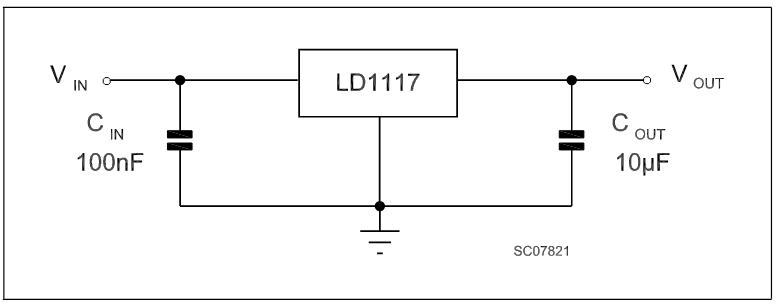
\includegraphics[width=1.0\linewidth]{voltageRegulation_3v3}
        \captionof{figure}{3.3 V Circuit \cite{datasheetLD1117}}
        \label{fig:voltageRegulation_3v3}
    \end{minipage}
    \begin{minipage}{.4\textwidth}
        \centering
        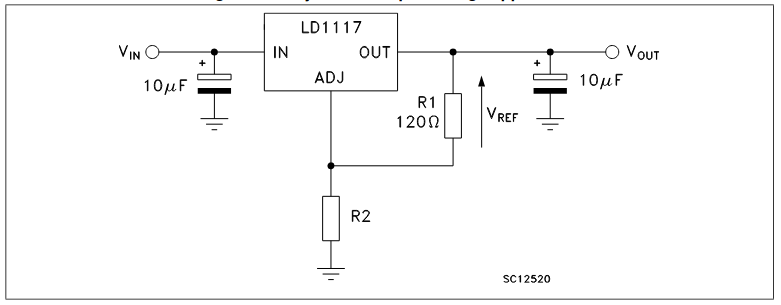
\includegraphics[width=1.0\linewidth]{voltageRegulation_5v}
        \captionof{figure}{5 V Circuit \cite{datasheetLD1117}}
        \label{fig:voltageRegulation_5v}
    \end{minipage}
\end{figure}

The feedback resistor values simply need to be calculated. According to \cite{datasheetLD1117}, $R_2$ in Figure \ref{fig:voltageRegulation_5v}
can be calculated using $V_{out} = V_{ref} (1 + \frac{R2}{R1})$. With $V_{out} = \SI{5}{V}$, $V_{ref} \approx \SI{1.25}{V}$, and $R_1 = \SI{120}{\ohm}$,
$R_2 = R_1 \cdot \left(\frac{V_{out}}{V_{ref}} - 1\right) = \SI{360}{\ohm}$. A $\SI{470}{\ohm}$ potentiometer will be used for the practical circuit to adjust the output to exactly $\SI{5}{V}$.

\pagebreak